\section{Results}\label{sec:results}
\subsection{Simulated turbulence}\label{sec:simulated}

To validate our algorithm, first we simulate atmospheric turbulence and try and directly measure wind speed without any interaction with the telescope optics. To do this, we emulate the procedure from \citet[sec.~4.1]{guyon_adaptive_2017}, which generates a phase screen with \SI{2}{\micro\meter} RMS wavefront error, which corresponds to a Fried parameter of $r_0=$\SI{20}{\centi\meter}, matching typical good seeing on Mauna Kea. Seven atmospheric layers are simulated using Von Karman statistics and summed together using the frozen-flow hypothesis \citep[see][tbl.~1]{guyon_adaptive_2017}. We simulated three different wind speeds, 3, 6, and \SI{10}{\meter\per\second}. For each simulation, we generate a cube with \num{10000} frames and measure offsets using Algorithm~\autoref{alg:windspeed}.

\begin{figure}
    \centering
    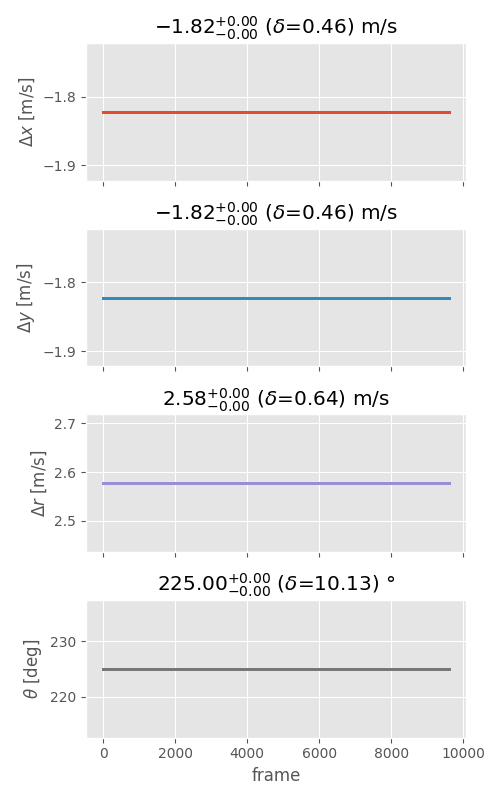
\includegraphics[width=0.32\textwidth]{chains_3ms}
    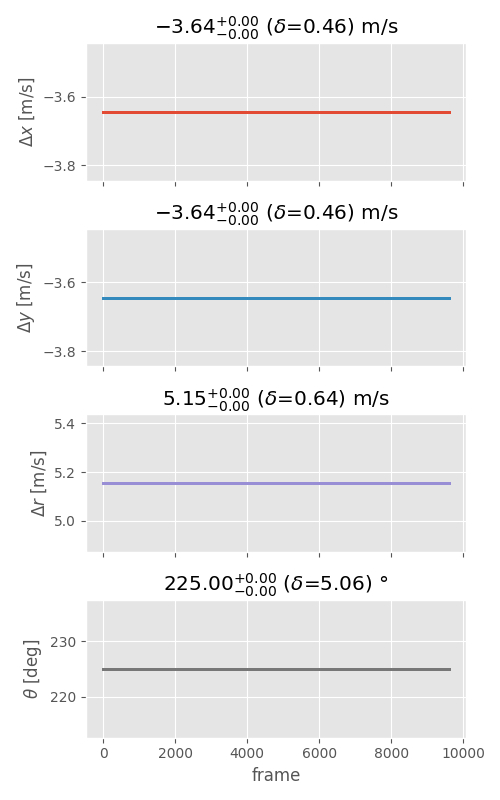
\includegraphics[width=0.32\textwidth]{chains_6ms}
    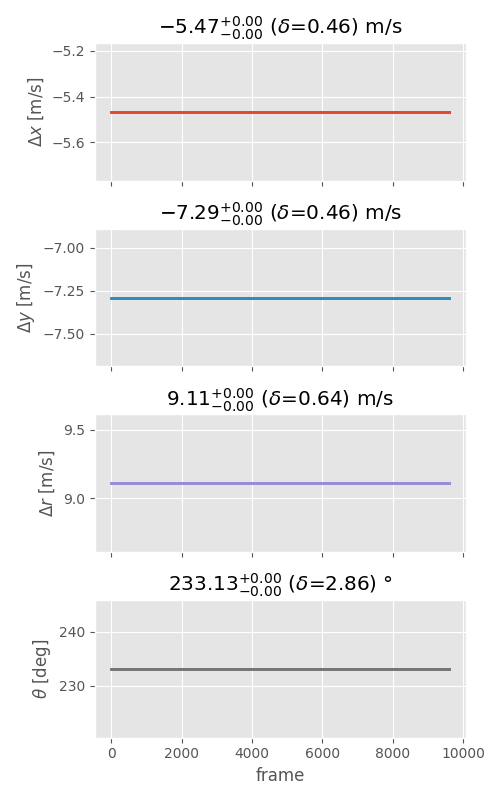
\includegraphics[width=0.32\textwidth]{chains_10ms}
    \caption{Offsets measured from simulated wavefront data. Printed above each chain is the median value, the spread of the inner quartile, and the resolution of the measurement. The offsets in $x$ and $y$ are the first two rows (red, blue). The vector magnitude $r$ and direction $\theta$ are the last two rows (purple, gray). The first column has \SI{3}{\meter\per\second} simulated wind speed. The second column has \SI{6}{\meter\per\second} simulated wind speed, and the last column has \SI{10}{\meter\per\second} simulated wind speed.}
    \label{fig:simulated}
\end{figure}

In \autoref{fig:simulated}, we can see the offsets measured by our algorithm on the simulated turbulence data. The magnitude of the wind speed for each cube (third row, purple) is very close to the true value. Any discrepancies here can be explained by slight differences in calibration (like the pupil platescale). The direction of the translation matches the visual flow in the input data.

\subsection{Simulated turbulence on the SCExAO testbed}\label{sec:turbulence}

The previous experiment does not include any details of the AO system or telescope optics. To address this, we further validate our algorithm on the SCExAO testbed \citep{guyon_wavefront_2011}. The testbed includes internal light sources which allow running the AO loop and taking data during off-hours. We use the testbed with the internal light source as a baseline for our next experiment. In this test, we take the simulated turbulence from \autoref{sec:turbulence} and manually inject the wavefront errors onto the deformable mirror. Once we have the AO loop running and the have adjusted the gain after injecting the wavefront errors, we again save a cube of 10,000 frames for analysis with Algorithm~\autoref{alg:windspeed}.

\begin{figure}
    \centering
    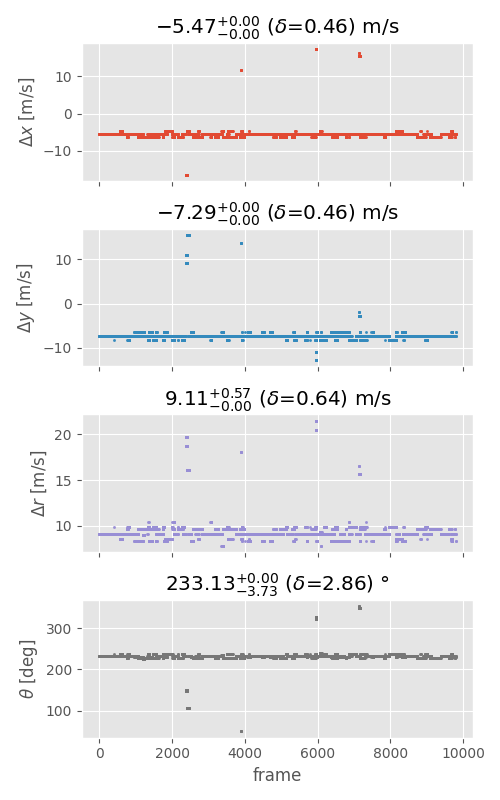
\includegraphics[width=0.35\textwidth]{chains_testbed}
    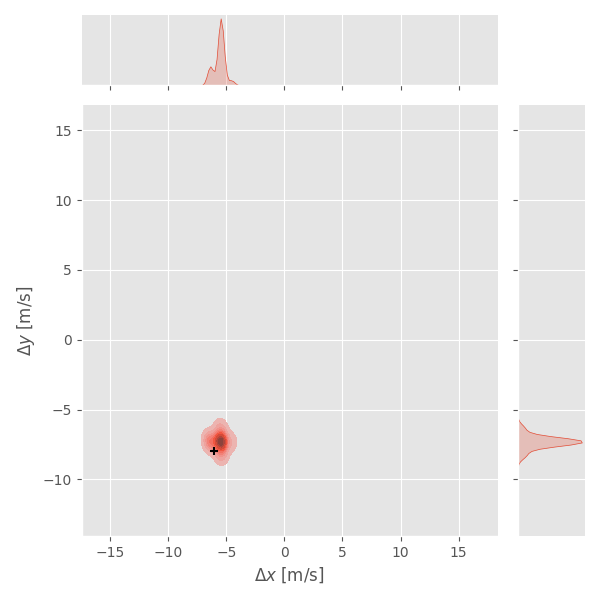
\includegraphics[width=0.5\textwidth]{radial_testbed}
    \caption{Offsets measured from injected turbulence with \SI{10}{\meter\per\second} wind speed on the SCExAO testbed using an internal light source. The left plots show chains for the offsets, while the right plot shows the kernel density estimate (KDE) of the measurements. Printed above each chain is the median value, the spread of the inner quartile, and the resolution of the measurement. The true value of \SI{10}{\meter\per\second} is marked by a cross in the 2-D KDE plot.}
    \label{fig:testbed}
\end{figure}

In \autoref{fig:testbed} we see that the \SI{10}{\meter\per\second} wind speed is recovered well, even with the added complexities of the SCExAO system. We are satisfied with the performance of the algorithm using simulated data on the testbed.

\subsection{On-sky SCExAO data}\label{sec:onsky}

In order to study the dynamics of wind speed, we need to apply our algorithm on-sky. The SCExAO team keep an archive of previous observations with saved AO telemetry. While not every observation includes the pseudo-open-loop telemetry we need for our algorithm, there are many half-nights with hours of the telemetry we need saved. Ideally, we could take the data cubes from each of these nights, apply our algorithm to them, and create a chain of wind speed measurements over many hours. These chains could then be analyzed for dynamic changes in the wind, such as the time scale for changing wind directions. These are the results we want to analyze for improving predictive control methods.

As a start, we found AO data that has a visible flow which may correspond to wind in the atmosphere. By visual inspection, the flow appears to have $\sim$\SI{3}{\pixel} motion over 200 frames at $\sim$ \SI{90}{\degree}. This data was taken while the AO loop was running at \SI{3.5}{\kilo\hertz}, so the corresponding wind speed is $\sim$\SI{9}{\meter\per\second}. Visibly this data suffers from far more systematics than the testbed data with regards to our algorithm. For example, on-sky data has a pronounced tip-tilt ``beating'', which is what inspired the modal filtering in Algorithm~\autoref{alg:windspeed}. In addition, the on-sky data is generally much noisier and often suffers from low-wind effect (LWE), which causes the quadrants in the pupil delimited by the secondary support spiders to ``petal" out. Spurious, noisy correlations dominate the outputs, shown in \autoref{fig:onsky}.

\begin{figure}
    \centering
    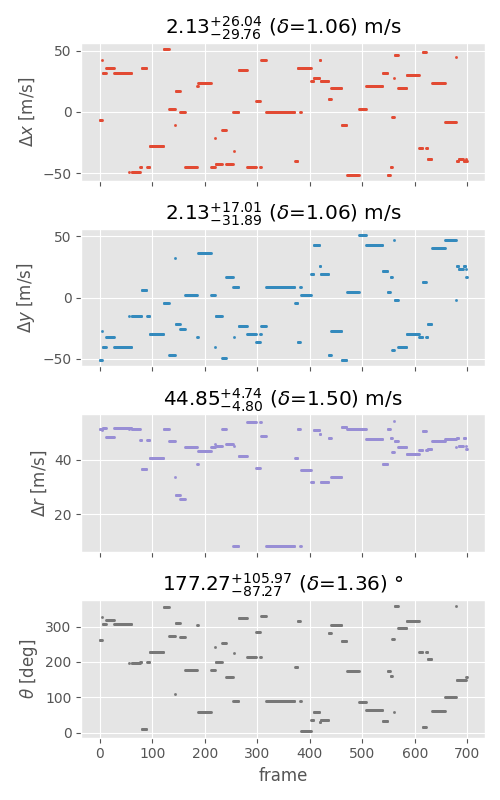
\includegraphics[width=0.35\textwidth]{chains_onsky}
    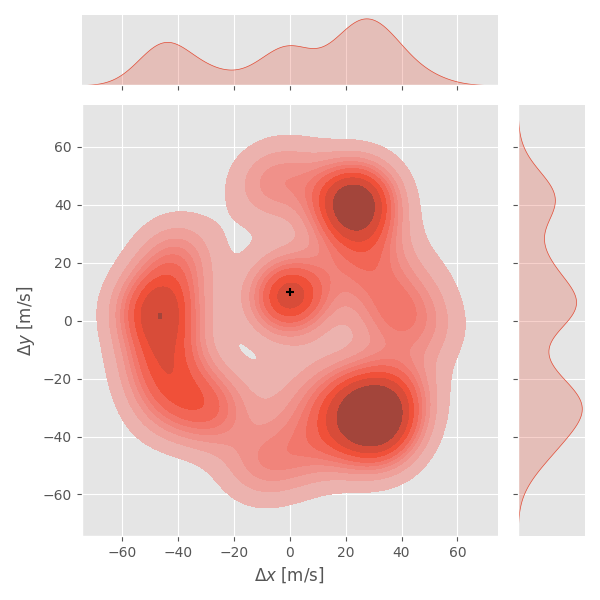
\includegraphics[width=0.5\textwidth]{radial_onsky}
    \caption{Offsets measured from on-sky SCExAO data. The left plots show chains for the offsets, while the right plot shows the 2-D marginal kernel density estimate (KDE) of the $x$ and $y$ measurements. Printed above each chain is the median value, the spread of the inner quartile, and the resolution of the measurement. The marginal KDE is cropped to only show detectable values according to \autoref{eqn:max}. The apparent motion between frames is marked with a black cross in the 2-D KDE plot.}
    \label{fig:onsky}
\end{figure}

The value we expected to retrieve is seen in the marginal distribution of \autoref{fig:onsky} ($\sim$\SI{9}{\meter\per\second} at \SI{90}{\degree}), which means our algorithm is working \textit{sometimes}. It is notable that the spurious offset measurements tend to occur in a ring close to the maximum detectable wind speed, which is even more pronounced if we do less aggressive modal and high-pass filtering.
